\chapter{Internet of Things \& Low-Power Wide-Area Networks}
\label{sec:chapter8}

The exponential proliferation of connected smart devices has established the Internet of Things (IoT) as a fundamental cornerstone of smart cities, automated utility metering, healthcare tele-monitoring, and Industry~4.0 industrial automation. However, IoT deployments encompass radically divergent application requirements, bifurcating modern medium access control (MAC) research into two dominant paradigms:
\begin{enumerate}
    \item \textbf{Cellular Low-Power Wide-Area Networks (LPWAN):} Designed to connect tens of thousands of uncoordinated, battery-constrained user equipments (UEs) per cell over multi-kilometer distances and deep indoor subterranean environments. The preeminent standard in this domain is the Third Generation Partnership Project (3GPP) \textbf{Narrowband Internet of Things (NB-IoT)}, operating over licensed cellular spectrum.
    \item \textbf{Deterministic Industrial IoT (IIoT):} Tailored for factory automation, robotic process control, and wireless sensor-actuator networks requiring deterministic microsecond-level latency, bounded jitter, and $99.999\%$ high reliability. The premier international standard is the \textbf{IEEE 802.15.4e Time Slotted Channel Hopping (TSCH)} protocol and the associated IETF \textbf{6TiSCH} protocol architecture.
\end{enumerate}

Both paradigms break down classical random access assumptions. In NB-IoT, traditional collision models fail to account for multi-tone coverage enhancement (CE) levels, repeated transmissions, and multi-band slotted ALOHA dynamics. In TSCH networks, strict time-slotted channel hopping eliminates external interference but introduces complex primary transceiver conflicts and multi-interferer secondary conflicts across routing topologies.

This chapter presents the comprehensive analytical models, optimization frameworks, and scheduling algorithms developed by Ramineni, Bommisetty, George, and Venkatesh \cite{ramineni2022performance, ramineni2019impact, bommisetty2022dplls, bommisetty2023cbpf, george2018performance, george2020multipacket}.

\section{Narrowband IoT (NB-IoT): Random Access and Coverage Enhancement}
\label{sec:nbiot_ra}

Introduced in 3GPP Release~13, Narrowband IoT (NB-IoT) is a cellular radio access technology specifically optimized for ultra-low device complexity, ultra-long battery life exceeding 10 years, and massive connection density ($> 52{,}547$ devices per cell site). A defining feature of NB-IoT is its capability to achieve an extreme link budget enhancement of up to $+20\text{~dB}$ over legacy GPRS, enabling communication through thick concrete walls and subterranean meter shafts.

\subsection{NB-IoT Radio Structure and NPRACH Architecture}
NB-IoT operates with a minimum system bandwidth of $180\text{~kHz}$, corresponding to exactly one LTE Physical Resource Block (PRB). It supports three deployment modes:
\begin{itemize}
    \item \textbf{Stand-alone:} Utilizing dedicated re-farmed GSM carrier frequencies.
    \item \textbf{Guard-band:} Utilizing the unused guard bands between adjacent LTE carriers.
    \item \textbf{In-band:} Utilizing resource blocks within an existing operational LTE carrier.
\end{itemize}

Uplink transmissions utilize the \textbf{Narrowband Physical Random Access Channel (NPRACH)}. In the frequency domain, the $180\text{~kHz}$ uplink bandwidth is partitioned into 48 subcarriers with a narrow subcarrier spacing of $3.75\text{~kHz}$ (or alternatively 12 subcarriers at $15\text{~kHz}$). Preamble transmissions consist of four symbol groups with frequency hopping; because the pseudo-random hopping sequence spans 12 subcarriers, subcarriers must be allocated in integer multiples of 12.

To guarantee service to devices experiencing heterogeneous signal attenuation, the cell is partitioned into three distinct \textbf{Coverage Enhancement (CE)} levels based on the Reference Signal Received Power (RSRP) measured by the UE:
\begin{itemize}
    \item \textbf{CE Level 0 (Normal Coverage):} High RSRP (devices close to the base station). Packets are transmitted with 1 preamble repetition and small back-off windows.
    \item \textbf{CE Level 1 (Robust Coverage):} Intermediate RSRP (indoor devices). Packets are transmitted with moderate repetitions (e.g., 2 to 8 repetitions).
    \item \textbf{CE Level 2 (Extreme Coverage):} Low RSRP (deep indoor subterranean utility meters). Preamble signals are repeated up to 32, 64, or 128 times to enable energy accumulation at the eNodeB receiver.
\end{itemize}

Let $S_0, S_1, S_2$ denote the number of subcarriers allocated to CE levels 0, 1, and 2, respectively. Subject to the 48-subcarrier total limit and the 12-subcarrier hopping constraint, permissible subcarrier allocation vectors include $\{12, 12, 12\}$, $\{24, 12, 12\}$, $\{12, 24, 12\}$, and $\{12, 12, 24\}$.

\subsection{Four-Step Contention-Based Random Access (CBRA) Procedure}
Random access in NB-IoT is contention-based and governs initial synchronization and uplink channel request:
\begin{enumerate}
    \item \textbf{Step 1: Preamble Transmission (Message 1):} After acquiring System Information Block 2 (SIB-2), the UE randomly selects one subcarrier from the $S_i$ subcarriers allocated to its current CE level $i$ and transmits its preamble sequence on the NPRACH.
    \item \textbf{Step 2: Random Access Response (Message 2):} The eNodeB monitors the NPRACH and replies with a Random Access Response (RAR) on the downlink control channel (NPDCCH/NPDSCH). The RAR contains the preamble identifier, timing advance, Temporary Cell Radio Network Temporary Identifier (TC-RNTI), and an uplink grant. The UE awaits RAR arrival within a configured RAR window timer.
    \item \textbf{Step 3: Scheduled Transmission (Message 3):} Using the allocated uplink grant, the UE transmits an RRC Connection Request containing its TC-RNTI and data payload size. If two or more UEs selected the identical subcarrier in Step~1, they decode the identical RAR and transmit on the same Message~3 resource, culminating in a Message~3 collision.
    \item \textbf{Step 4: Contention Resolution (Message 4):} The eNodeB transmits the Contention Resolution message containing the unique identity of the winning UE. If the UE receives Message~4 prior to timer expiration, random access succeeds; otherwise, collision is declared, and the UE triggers back-off.
\end{enumerate}

\subsection{Two-Counter Mechanism and Coverage Enhancement Migration}
NB-IoT standardizes a dual-counter mechanism to manage preamble retransmissions:
\begin{enumerate}
    \item \textbf{Overall Preamble Attempt Counter:} Increments after every unsuccessful attempt across all CE levels, bounded by the cell-wide ceiling $M$.
    \item \textbf{CE-Level Counter:} Counts attempts within the current CE level, bounded by the level-specific ceiling $R_i$.
\end{enumerate}

When the CE-level counter reaches $R_i$ before the overall counter reaches $M$, the UE resets the CE-level counter to zero and migrates to the next higher CE level $i+1$, increasing its repetition count and transmit power.

For a UE whose initial channel measurement placed it in CE level $x$, the maximum number of attempts permitted in subsequent CE level $y$ ($y \ge x$) is derived by Ramineni et al. \cite{ramineni2022performance} as:
\begin{equation}
    \label{eq:R_xy_migration}
    R_{xy} = \max\left(0, \, \min\left(R_y, \, M - \sum_{b=x}^{y-1} R_b\right)\right), \qquad 0 \le x \le y \le 2
\end{equation}

\subsection{Three-Dimensional Markov Chain Model for NB-IoT UEs}
To capture the coupling between back-off counters, retransmission stages, and inter-CE migrations, Ramineni, Venkatesh, and Bommisetty \cite{ramineni2022performance} developed a 3-dimensional Discrete-Time Markov Chain (DTMC). The state of a contending UE is modeled as a 3-tuple:
\begin{equation}
    (i, j, k)
\end{equation}
where:
\begin{itemize}
    \item $i \in \{0, 1, 2\}$ denotes the active CE level,
    \item $j \in \{1, 2, \dots, R_{xy}\}$ denotes the preamble transmission attempt counter within the current CE level,
    \item $k \in \{0, 1, \dots, W_i - 1\}$ denotes the back-off counter, where $W_i$ is the back-off window size in units of NPRACH periodic slots $\delta_i$.
\end{itemize}

Figure~\ref{fig:nbiot_markov_ce0} depicts the complete state transition diagram for a UE that initiates its random access procedure in CE level~0.

\begin{figure}[htbp]
    \centering
    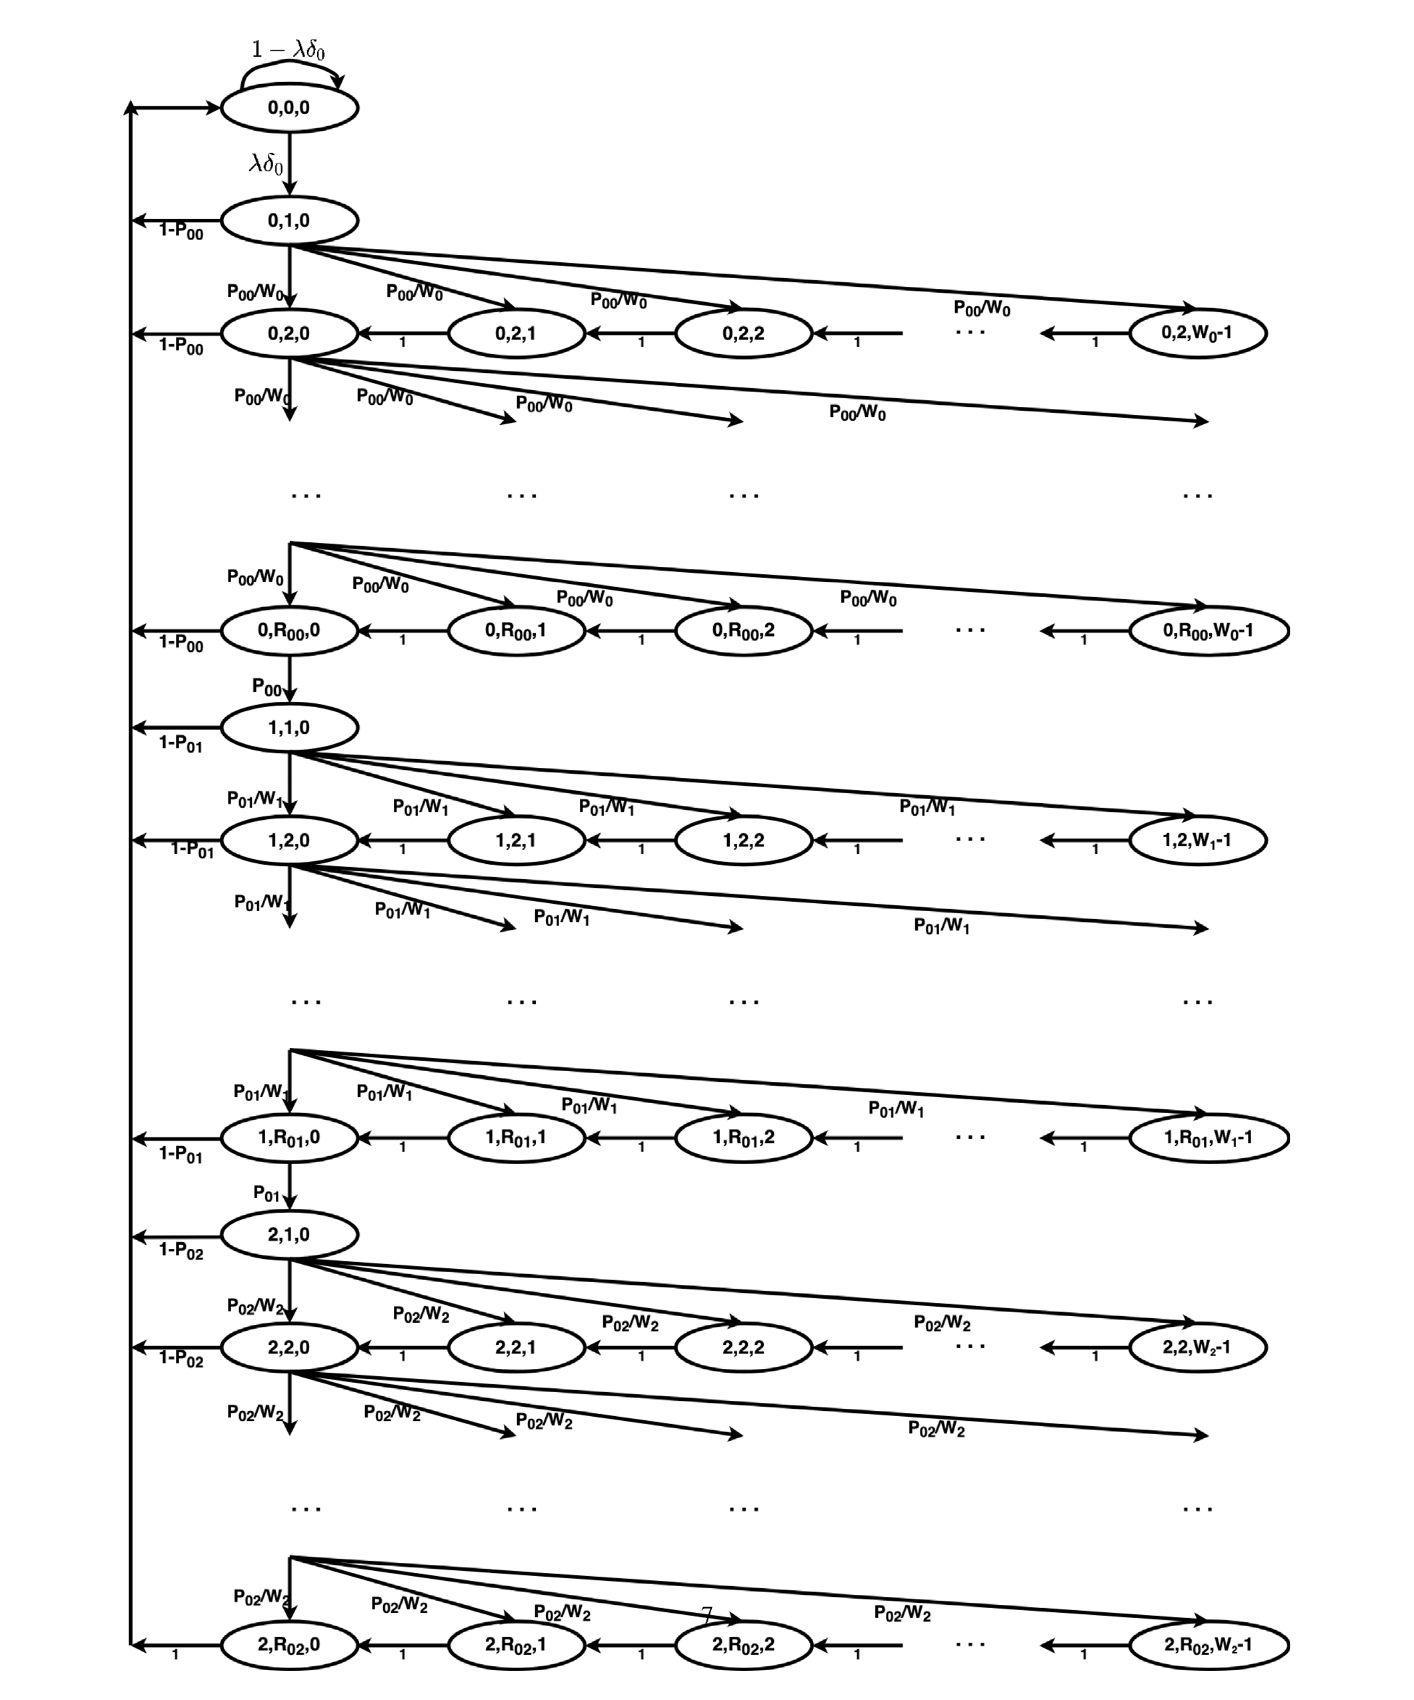
\includegraphics[width=0.98\textwidth]{figures/fig_nbiot_markov_ce0.png}
    \caption{Three-dimensional Discrete-Time Markov Chain model for NB-IoT UEs initiating random access in Coverage Enhancement level 0 (CE~0) and migrating to CE~1 and CE~2 \cite{ramineni2022performance}.}
    \label{fig:nbiot_markov_ce0}
\end{figure}

The state $(0, 0, 0)$ represents the power-saving \textbf{Idle state}, where the device sleeps awaiting a packet arrival. Assuming packet arrivals follow a Poisson process with average arrival rate $\lambda$, the probability of a packet arriving during an idle slot of length $\delta_0$ is $\lambda \delta_0$ (under standard Bernoulli discretization for small $\lambda \delta_0$).

\subsubsection{State Transition Probabilities for CE Level 0}
Upon packet arrival, the UE transitions to state $(0, 1, 0)$ and transmits its initial preamble:
\begin{equation}
    \pi_{0,1,0} = \pi_{0,0,0} \lambda \delta_0
\end{equation}
If the transmission collides with probability $p_{00}$, the UE enters back-off stage $j = 2$:
\begin{equation}
    \pi_{0,2,0} = \pi_{0,1,0} p_{00} = \pi_{0,0,0} p_{00} \lambda \delta_0
\end{equation}

For any back-off slot $k \in \{0, \dots, W_0 - 1\}$ during attempt $j \in \{2, \dots, R_{00}\}$:
\begin{equation}
    \pi_{0,j,k} = \pi_{0,j,k+1} + \pi_{0,j-1,0} \frac{p_{00}}{W_0} = \frac{W_0 - k}{W_0} \pi_{0,j-1,0} p_{00}
\end{equation}
Repeated substitution yields:
\begin{equation}
    \pi_{0,j,k} = \frac{W_0 - k}{W_0} p_{00}^{j-1} \lambda \delta_0 \pi_{0,0,0}, \qquad 2 \le j \le R_{00}
\end{equation}

\subsubsection{CE Migration Transition to CE Level 1 and CE Level 2}
When a UE exhausts its maximum permitted attempts $R_{00}$ in CE level 0 without success, it migrates to CE level 1. Its initial attempt in CE level 1 is governed by:
\begin{equation}
    \pi_{1,1,0} = \pi_{0, R_{00}, 0} p_{00} = p_{00}^{R_{00}} \lambda \delta_0 \pi_{0,0,0}
\end{equation}
Within CE level 1, the back-off window is $W_1$ and collision probability is $p_{01}$. The state probabilities become:
\begin{equation}
    \pi_{1,j,k} = \frac{W_1 - k}{W_1} p_{00}^{R_{00}} p_{01}^{j-1} \lambda \delta_0 \pi_{0,0,0}, \qquad 2 \le j \le R_{01}
\end{equation}

Similarly, if contention fails after $R_{01}$ attempts in CE level 1, the UE migrates to CE level 2:
\begin{equation}
    \pi_{2,1,0} = \pi_{1, R_{01}, 0} p_{01} = p_{00}^{R_{00}} p_{01}^{R_{01}} \lambda \delta_0 \pi_{0,0,0}
\end{equation}
\begin{equation}
    \pi_{2,j,k} = \frac{W_2 - k}{W_2} p_{00}^{R_{00}} p_{01}^{R_{01}} p_{02}^{j-1} \lambda \delta_0 \pi_{0,0,0}, \qquad 2 \le j \le R_{02}
\end{equation}

\subsubsection{Normalization Condition}
Every state probability $\pi_{i,j,k}$ is expressed linearly in terms of the idle state probability $\pi_{0,0,0}$. The total probability conservation law enforces:
\begin{equation}
    \label{eq:nbiot_normalization}
    \pi_{0,0,0} + \sum_{j=1}^{R_{00}} \sum_{k=0}^{W_0-1} \pi_{0,j,k} + \sum_{j=1}^{R_{01}} \sum_{k=0}^{W_1-1} \pi_{1,j,k} + \sum_{j=1}^{R_{02}} \sum_{k=0}^{W_2-1} \pi_{2,j,k} = 1
\end{equation}
Evaluating the summations provides a closed-form solution for the idle probability $\pi_{0,0,0}$:
\begin{align}
    \pi_{0,0,0}^{-1} = 1 &+ \lambda \delta_0 \left[ 1 + \frac{W_0 + 1}{2} \sum_{j=2}^{R_{00}} p_{00}^{j-1} \right] \nonumber \\
    &+ \lambda \delta_0 p_{00}^{R_{00}} \left[ 1 + \frac{W_1 + 1}{2} \sum_{j=2}^{R_{01}} p_{01}^{j-1} \right] \nonumber \\
    &+ \lambda \delta_0 p_{00}^{R_{00}} p_{01}^{R_{01}} \left[ 1 + \frac{W_2 + 1}{2} \sum_{j=2}^{R_{02}} p_{02}^{j-1} \right]
\end{align}

Similar closed-form Markov models are derived for UEs initiating access directly in CE level 1 and CE level 2 \cite{ramineni2022performance}.

\subsection{Transmission Probability, Collision Probability, and System Throughput}
A preamble transmission occurs whenever a UE occupies a state with back-off counter $k = 0$. For a UE initially in CE level $i$ transmitting in CE level $j$, the slot transmission probability is:
\begin{equation}
    \tau_{ij} = \sum_{k=1}^{R_{ij}} \pi_{j, k, 0}
\end{equation}
The aggregate transmission probability of any active UE in CE level $j$ across all UE cohorts is:
\begin{equation}
    \tau_j = \sum_{i=0}^j \tau_{ij}
\end{equation}

When $N_j$ UEs contend over $S_j$ orthogonal subcarriers, a tagged preamble transmission succeeds if and only if none of the remaining $N_j - 1$ UEs transmit on the same subcarrier in that slot. Hence, the conditional preamble collision probability is:
\begin{equation}
    p_{ij} = 1 - \left( 1 - \frac{\tau_j}{S_j} \right)^{N_j - 1}
\end{equation}
This system of coupled non-linear equations for $\{\tau_j, p_{ij}\}$ is solved numerically using fixed-point iteration.

The unconditional probability of successful packet delivery in CE level $j$ for a UE initially in CE level $i$ after $k$ attempts is:
\begin{equation}
    p_{s,ijk} = (1 - p_{ij}) p_{ij}^{k-1} \prod_{b=i}^{j-1} p_{ib}^{R_{ib}}
\end{equation}

Finally, the MAC layer throughput $T_i$ (in packets delivered per second) for UEs belonging to initial CE group $i$ is:
\begin{equation}
    \label{eq:nbiot_throughput}
    T_i = \frac{1}{\delta_i} \sum_{j=i}^2 \sum_{k=1}^{R_{ij}} \pi_{j,k,0} (1 - p_{ij})
\end{equation}

\subsection{Subcarrier Allocation Optimization in Heterogeneous Demographics}
Ramineni et al. \cite{ramineni2022performance} evaluated system throughput across different subcarrier configurations $\{S_0, S_1, S_2\}$:
\begin{itemize}
    \item \textbf{Urban Macrocells (Dominated by CE 0):} With $80\%$ of devices in CE 0, the allocation $\{24, 12, 12\}$ yields over $45\%$ higher throughput than the uniform $\{12, 12, 12\}$ allocation. Because CE 0 uses no repetitions, granting it 24 subcarriers maximizes total delivered packets per second.
    \item \textbf{Subterranean / Rural Environments (Dominated by CE 2):} When deep-indoor smart meters dominate, allocating 24 subcarriers to CE 2 ($\{12, 12, 24\}$) is essential. Without adequate subcarrier allocation, long repetition durations saturate CE 2 subcarriers, causing complete random access collapse and cascading battery exhaustion.
\end{itemize}

\section{Access Class Barring (ACB) Congestion Control in NB-IoT}
\label{sec:nbiot_acb}

Due to the massive density of IoT installations ($10^5\text{~devices/km}^2$), external triggers such as power grid fluctuations or earthquake sensor alerts can cause tens of thousands of UEs to synchronize and transmit preambles simultaneously. This triggers severe RACH overload, where NPRACH collisions approach $100\%$, locking the channel in gridlock.

To mitigate RACH overload, Ramineni and Venkatesh \cite{ramineni2019impact} investigated the adaptation of \textbf{Access Class Barring (ACB)} for NB-IoT.

\subsection{Access Class Barring Mechanism}
In ACB, the eNodeB broadcasts two critical control parameters inside SIB-2:
\begin{itemize}
    \item \textbf{Access Barring Factor ($\alpha_{\text{acb}} \in [0, 1]$):} The probability that a device is granted immediate access.
    \item \textbf{Access Barring Time ($T_{\text{acb}}$):} The base duration for which barred devices must suppress transmission.
\end{itemize}

Before initiating Step~1 of random access, a UE generates a uniform pseudo-random number $U \sim \mathcal{U}[0, 1]$:
\begin{itemize}
    \item If $U \le \alpha_{\text{acb}}$, the UE passes the barring check and immediately transmits its preamble on NPRACH.
    \item If $U > \alpha_{\text{acb}}$, the UE is barred from channel access. The UE must back off for a randomized duration $T_{\text{barring}}$ before re-evaluating access:
    \begin{equation}
        T_{\text{barring}} = \left( 0.7 + 0.6 \, U_{\text{rand}} \right) T_{\text{acb}}, \qquad U_{\text{rand}} \sim \mathcal{U}[0, 1]
    \end{equation}
\end{itemize}

\subsection{Performance Impact of Dynamic ACB Tuning}
Ramineni and Venkatesh \cite{ramineni2019impact} demonstrated that while 3GPP standards initially favored Extended Access Barring (EAB) over ACB for NB-IoT, dynamic broadcasting of the ACB factor $\alpha_{\text{acb}}$ delivers superior stability under bursty Beta traffic. By throttling initial access ($\alpha_{\text{acb}} \approx 0.2$ to $0.4$ during peak arrivals), preamble collision rates on NPRACH drop from over $85\%$ to below $15\%$. Consequently, the total access completion time of the network is halved, and individual battery drain per successful connection is reduced by over $60\%$.

\section{Industrial IoT: IEEE 802.15.4e Time Slotted Channel Hopping (TSCH)}
\label{sec:tsch_fundamentals}

While cellular NB-IoT addresses wide-area connectivity, mission-critical factory automation and process control mandate deterministic, ultra-reliable communication over short-range mesh networks. The **IEEE 802.15.4e** standard introduced the **Time Slotted Channel Hopping (TSCH)** MAC mode to eliminate the vulnerabilities of unslotted CSMA/CA in industrial environments.

\subsection{TSCH Principles: Slotframes, Cells, and Frequency Hopping}
In TSCH, time is discretized into fixed-duration time slots (typically $10\text{~ms}$), sufficient to transmit a maximum-length PHY frame (127 bytes) and receive an acknowledgment (ACK).

Time slots are grouped into a repeating cycle called a \textbf{slotframe} of length $N_{\text{slot}}$. Transmissions are allocated over a two-dimensional grid indexed by $(\text{timeslot}, \text{channelOffset})$, termed a \textbf{cell}:
\begin{itemize}
    \item \textbf{Timeslot:} The relative position within the slotframe ($0 \le t < N_{\text{slot}}$).
    \item \textbf{Channel Offset:} A logical index ($0 \le \text{ch} < M$), where $M \le 16$ is the number of available physical channels in the $2.4\text{~GHz}$ ISM band.
\end{itemize}

To overcome multi-path Rayleigh fading and external narrow-band interference (e.g., co-located Wi-Fi networks), TSCH executes pseudo-random frequency hopping at every time slot. The physical communication frequency $f$ assigned to a cell is computed dynamically via:
\begin{equation}
    \label{eq:tsch_channel_hopping}
    f = F\left( (\text{ASN} + \text{channelOffset}) \bmod M \right)
\end{equation}
where $\text{ASN}$ (Absolute Slot Number) is a globally synchronized 5-byte counter that increments monotonically at every time slot since network initialization, and $F(\cdot)$ is a pre-shared lookup table mapping logical offsets to physical channel frequencies (IEEE 802.15.4 channels 11 to 26).

\subsection{The 6TiSCH Architecture and RPL Routing}
To seamlessly integrate TSCH with IPv6 industrial IoT ecosystems, the IETF formed the **6TiSCH** working group. The protocol stack incorporates:
\begin{itemize}
    \item \textbf{RPL (Routing Protocol for Low-Power and Lossy Networks):} Constructs a Destination-Oriented Directed Acyclic Graph (DODAG) tree topology $T = (V, E_T)$ rooted at a centralized 6LBR (6LoWPAN Border Router). Each node $i \in V$ identifies its preferred parent $p(i) \in V$ and forwards sensor telemetry over multi-hop tree links.
    \item \textbf{6top Sublayer:} Sits between the IEEE 802.15.4e TSCH MAC and the network layer, responsible for dynamically scheduling cells and negotiating link resource allocations.
\end{itemize}

\subsection{Conflict Taxonomy in TSCH Networks}
As formulated by Bommisetty and Venkatesh \cite{bommisetty2022dplls, bommisetty2023cbpf}, transmissions in a TSCH network are subject to two fundamental physical conflicts, illustrated in Figure~\ref{fig:cbpf_conflicts}:

\begin{figure}[htbp]
    \centering
    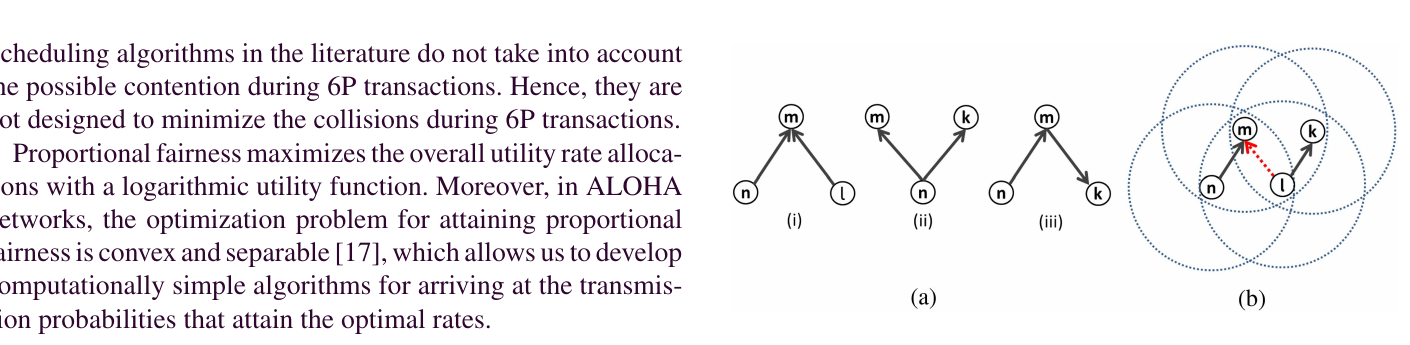
\includegraphics[width=0.92\textwidth]{figures/fig_cbpf_conflicts.png}
    \caption{Classification of conflicts in TSCH networks: (a) Primary conflicting links (half-duplex transceiver constraints), (b) Secondary conflicting links (co-channel interference within the interference radius) \cite{bommisetty2023cbpf}.}
    \label{fig:cbpf_conflicts}
\end{figure}

\begin{enumerate}
    \item \textbf{Primary Conflicts:} Arise from half-duplex hardware constraints of low-cost IoT transceivers. A node cannot simultaneously transmit and receive, nor can it transmit to or receive from two distinct nodes concurrently. The set of links in primary conflict with a given link $(n, m)$ is:
    \begin{equation}
        I_{nm}^p = \left\{ (l, k) \in \mathcal{S} \;\Big|\; \{l, k\} \cap \{n, m\} \ne \emptyset \right\}
    \end{equation}
    Transmissions on primary conflicting links cannot occur in the same time slot, even if assigned different channel offsets.
    \item \textbf{Secondary Conflicts:} Arise when two independent transmissions occur in the same time slot and on the identical physical channel within mutual interference range:
    \begin{equation}
        I_{nm}^s = \left\{ (l, k) \in \mathcal{S} \;\Big|\; m \in \mathcal{N}_l \;\lor\; k \in \mathcal{N}_n \right\}
    \end{equation}
    where $\mathcal{N}_n$ denotes the set of nodes within the interference range of node $n$. Transmissions on secondary conflicting links ($I_{nm}^s \setminus I_{nm}^p$) can occur concurrently in the same time slot, provided they are assigned distinct channel offsets.
\end{enumerate}

\section{Dynamic Programming Low-Latency Schedule (DPLLS) for 6TiSCH}
\label{sec:dplls}

Standard 6TiSCH scheduling protocols (such as 6P or minimal scheduling) incur substantial end-to-end buffering delays due to uncoordinated cell placement across successive hops. To achieve deterministic low latency, Bommisetty and Venkatesh \cite{bommisetty2022dplls} proposed **DPLLS (Dynamic Programming based Low-Latency Schedule)**.

\subsection{Generalised Conflict Graph (GCG)}
Conventional pairwise conflict graphs only capture interference between pairs of transmitters. However, in wireless networks, multiple weak transmissions can collectively degrade the Signal-to-Interference-plus-Noise Ratio (SINR) at a tagged receiver below the demodulation threshold $\alpha$, even when each individual transmitter is harmless.

To model aggregate sum-interference, Bommisetty and Venkatesh defined the \textbf{Generalised Conflict Graph (GCG)} $B(\mathcal{P}_V, E_B)$, where $\mathcal{P}_V$ is the power set of network nodes $V$. An hyper-edge $(i, \mathcal{I}) \in E_B$ exists between node $i$ and subset $\mathcal{I} \subseteq V$ if and only if:
\begin{equation}
    \text{SINR}\left((i, p(i)), \, \mathcal{I}\right) = \frac{P(i, p(i))}{N_{P, p(i)} + \sum_{j \in \mathcal{I}} P(j, p(i))} < \alpha
\end{equation}
where $P(x, y)$ is the received signal power at node $y$ when node $x$ transmits, and $N_{P, y}$ is receiver background noise.

\begin{figure}[htbp]
    \centering
    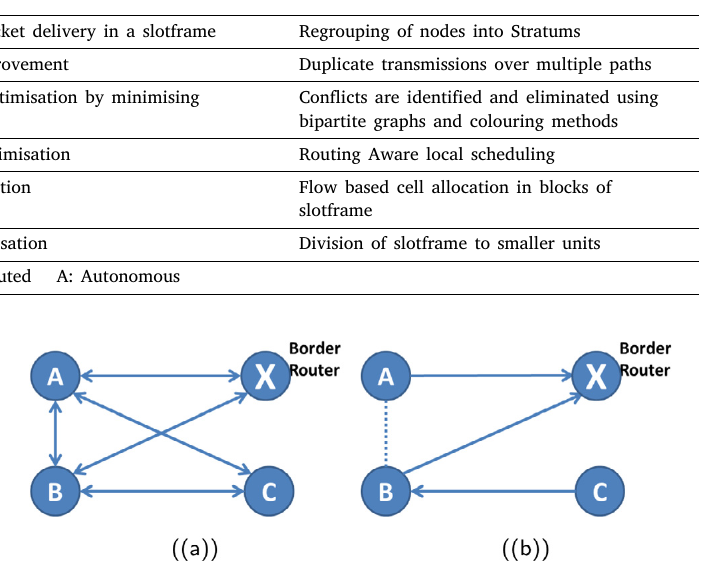
\includegraphics[width=0.75\textwidth]{figures/fig_dplls_network_topology.png}
    \caption{Example TSCH network model: (a) Physical network connectivity graph $G(V, E)$, (b) RPL-constructed Destination-Oriented Directed Acyclic Graph (DODAG) tree topology $T(V, E_T)$ \cite{bommisetty2022dplls}.}
    \label{fig:dplls_topology}
\end{figure}

\subsection{Maximum Weight Independent Set (MWIS) via Dynamic Programming}
DPLLS transforms the problem of eliminating primary conflicts while prioritizing heavily loaded nodes into the **Maximum Weight Independent Set (MWIS)** problem on the RPL DODAG tree $T = (V, E_T)$ (Figure~\ref{fig:dplls_topology}).

Let $w_i = Q(i)$ represent the weight of node $i$, defined as its instantaneous packet queue length. For each subtree $T_i$ rooted at node $i$, two recursive quantities are introduced:
\begin{align}
    M(i) &= \max\left\{ w(\mathcal{S}) \;\big|\; \mathcal{S} \text{ is an independent set in } T_i \text{ and } i \in \mathcal{S} \right\} \\
    M'(i) &= \max\left\{ w(\mathcal{S}) \;\big|\; \mathcal{S} \text{ is an independent set in } T_i \text{ and } i \notin \mathcal{S} \right\}
\end{align}

Because $T$ is cycle-free, $M(i)$ and $M'(i)$ are computed in a single bottom-up sweep from leaf nodes to the root border router:
\begin{align}
    \label{eq:mwis_dp_recursion}
    M(i) &= w_i + \sum_{j \in c(i)} M'(j) \\
    M'(i) &= \sum_{j \in c(i)} \max\left( M(j), \, M'(j) \right)
\end{align}
where $c(i)$ denotes the set of immediate children of node $i$ in the DODAG tree.

The global maximum weight independent set of $T$ is given by:
\begin{equation}
    \mathcal{S}^* = \arg\max\left( M(\text{root}), \, M'(\text{root}) \right)
\end{equation}
This dynamic programming recursion solves the MWIS on trees in strictly linear time $\mathcal{O}(|V|)$, completely eliminating primary conflicts in each scheduled time slot.

\subsection{DPLLS Algorithm Architecture and Block Scheduling}
The complete operational flow of DPLLS is illustrated in Figure~\ref{fig:dplls_block_diagram}:

\begin{figure}[htbp]
    \centering
    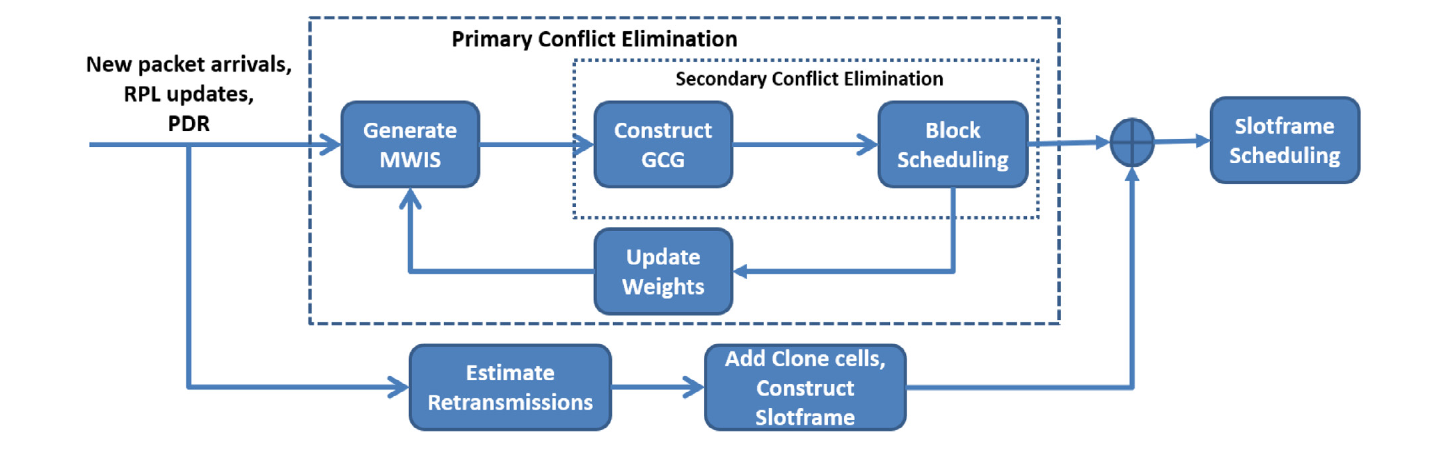
\includegraphics[width=0.95\textwidth]{figures/fig_dplls_block_diagram.png}
    \caption{Functional block diagram of the DPLLS scheduling architecture for 6TiSCH industrial networks \cite{bommisetty2022dplls}.}
    \label{fig:dplls_block_diagram}
\end{figure}

The algorithm executes the following sequence:
\begin{enumerate}
    \item \textbf{MWIS Generation:} Solves the tree DP recursion (\ref{eq:mwis_dp_recursion}) to find the optimal set of nodes that can transmit concurrently in a given slot without primary conflicts.
    \item \textbf{Secondary Conflict Elimination (GCG Construction):} Constructs the GCG of the active set $\mathcal{S}^*$ and assigns distinct channel offsets $(0, \dots, M-1)$ to resolve multi-interferer secondary conflicts.
    \item \textbf{Block Scheduling:} Grouping non-conflicting slots into a minimal repetitive unit called a \textbf{block}.
    \item \textbf{Retransmission Estimation and Slotframe Replication:} To guarantee end-to-end reliability over lossy wireless links, the number of retransmissions required on link $e = (i, p(i))$ to satisfy a target delivery reliability $R_{\text{target}}$ (e.g., $99.9\%$) is computed from its measured Packet Delivery Ratio ($\text{PDR}_e$):
    \begin{equation}
        N_{\text{retx}}(e) = \left\lceil \frac{\ln(1 - R_{\text{target}})}{\ln(1 - \text{PDR}_e)} \right\rceil
    \end{equation}
    The base block is replicated across the slotframe to accommodate these dedicated retransmission opportunities.
\end{enumerate}

By organizing the slotframe into tightly pipelined blocks, DPLLS minimizes the buffering delay between successive parent-child hops, reducing end-to-end packet delivery latency by up to $68\%$ compared to the 6TiSCH minimal configuration.

\section{Contention-Based Proportional Fairness (CBPF) in TSCH}
\label{sec:cbpf}

While scheduled TSCH guarantees bounded latency for periodic telemetry, bursty industrial alarms and aperiodic events require flexible, contention-based access. In IEEE 802.15.4e, shared cells allow multiple nodes to contend over the same $(\text{timeslot}, \text{channelOffset})$ using slotted ALOHA.

Bommisetty and Venkatesh \cite{bommisetty2023cbpf} developed the \textbf{Contention-Based Proportional Fairness (CBPF)} transmission scheme, establishing a convex optimization framework to maximize system throughput while guaranteeing fair resource distribution among competing IoT nodes.

\subsection{Link Success Probability Model}
Consider a TSCH network modeled as a multichannel slotted ALOHA system over $M$ orthogonal channels. Each node $n$ transmits a packet to destination $m \in \mathcal{D}_n$ with link transmission probability $\tau_{nm}$ and selects a physical channel uniformly at random with probability $1/M$.

Accounting for primary and secondary conflicts, the probability that transmission on directed link $(n, m)$ is successful in a generic time slot is derived in \cite{bommisetty2023cbpf} as:
\begin{equation}
    \label{eq:cbpf_link_success}
    \mu_{nm}(\boldsymbol{\tau}) = \tau_{nm} \prod_{(l, k) \in I_{nm}^p} (1 - \tau_{lk}) \prod_{(l, k) \in I_{nm}^s \setminus I_{nm}^p} \left( 1 - \frac{\tau_{lk}}{M} \right)
\end{equation}
In (\ref{eq:cbpf_link_success}):
\begin{itemize}
    \item The first product enforces silence across all primary conflicting links ($I_{nm}^p$), ensuring neither $n$ nor $m$ is involved in another transmission.
    \item The second product enforces channel isolation across secondary conflicting links ($I_{nm}^s \setminus I_{nm}^p$), ensuring that any concurrent transmission in the interference neighborhood selects a different physical channel (probability $1 - 1/M$).
\end{itemize}

\subsection{Proportional Fairness Optimization Formulation}
To incorporate queue status into scheduling, each link $(n, m)$ is assigned a dynamic weight as an increasing, concave function of its queue length $Q_{nm}$:
\begin{equation}
    w_{nm} = \log\left( 1 + Q_{nm} \right)
\end{equation}

Proportional fairness is achieved by finding the transmission probability vector $\boldsymbol{\tau}^*$ that maximizes the weighted log-utility of link success rates:
\begin{equation}
    \max_{\boldsymbol{\tau} \in \mathcal{P}} \sum_{(n, m) \in \mathcal{S}} w_{nm} \log \mu_{nm}(\boldsymbol{\tau})
\end{equation}

In a data collection network where $N$ sensor nodes transmit directly or via designated relays to a border router over $M$ channels, all links are in mutual interference conflict. The success probability of link $i \in \{1, \dots, N\}$ simplifies to:
\begin{equation}
    \mu_i = \tau_i \prod_{j=1, j \ne i}^N \left( 1 - \frac{\tau_j}{M} \right)
\end{equation}

The primal optimization problem is formulated as:
\begin{align}
    \label{eq:cbpf_optimization}
    \min_{\boldsymbol{\tau}} \quad & F(\boldsymbol{\tau}) = -\sum_{i=1}^N w_i \log \mu_i \nonumber \\
    \text{subject to} \quad & \sum_{i=1}^N \tau_i \le M, \qquad 0 \le \tau_i \le 1, \; \forall i \in \{1, \dots, N\}
\end{align}

\subsection{Lagrangian Duality and Closed-Form KKT Solution}
The objective function $F(\boldsymbol{\tau})$ is strictly convex over the hypercube $\mathcal{P}$, and the constraint is linear. Therefore, strong duality holds by Slater's condition. The Lagrangian function is:
\begin{equation}
    \mathcal{L}(\boldsymbol{\tau}, \gamma) = -\sum_{i=1}^N w_i \log \mu_i + \gamma \left( \sum_{i=1}^N \tau_i - M \right)
\end{equation}
where $\gamma \ge 0$ is the Lagrange multiplier.

Applying the Karush-Kuhn-Tucker (KKT) stationarity condition $\frac{\partial \mathcal{L}}{\partial \tau_i} = 0$:
\begin{equation}
    -\frac{w_i}{\tau_i} + \sum_{j=1, j \ne i}^N \frac{w_j}{M - \tau_j} + \gamma = 0
\end{equation}
Rearranging terms yields a quadratic equation in the optimal transmission probability $\tau_i^*$ for node $i$:
\begin{equation}
    \label{eq:cbpf_quadratic}
    \gamma (\tau_i^*)^2 - \left( \gamma M - \sum_{j=1}^N w_j \right) \tau_i^* + w_i M = 0
\end{equation}

The unique root of (\ref{eq:cbpf_quadratic}) that lies in $[0, 1]$ determines $\tau_i^*(\gamma)$, and the optimal dual variable $\gamma^*$ is obtained efficiently via one-dimensional bisection or gradient descent.

\subsection{Stochastic Performance Analysis of CBPF}
Because nodes have heterogeneous queue lengths $w_i$, their optimal transmission probabilities $\tau_i^*$ are non-identical. Consequently, the number of nodes attempting transmission in a slot does not follow a classical binomial distribution.

\subsubsection{Distribution of Transmitting Nodes via DFT}
Let $I_j \in \{0, 1\}$ be the transmission indicator for node $j$, with $P(I_j = 1) = \tau_j$. The characteristic function of $I_j$ is $\phi_{I_j}(t) = 1 - \tau_j + \tau_j e^{\mathrm{i} t}$ (where $\mathrm{i} = \sqrt{-1}$). The characteristic function of the total transmitting nodes $K = \sum_{j=1}^N I_j$ is:
\begin{equation}
    \phi_K(t) = \prod_{j=1}^N \left( 1 - \tau_j + \tau_j e^{\mathrm{i} t} \right)
\end{equation}

By evaluating $\phi_K(t)$ at the roots of unity $t = \frac{2\pi l}{N+1}$ and applying the Inverse Discrete Fourier Transform (IDFT), Bommisetty and Venkatesh \cite{bommisetty2023cbpf} derived the exact Probability Mass Function (PMF) $P_t(k; N)$ that exactly $k$ out of $N$ nodes transmit:
\begin{equation}
    P_t(k; N) = \frac{1}{N+1} \sum_{l=0}^N \left[ \prod_{j=1}^N \left( 1 - \tau_j + \tau_j e^{\mathrm{i} \frac{2\pi l}{N+1}} \right) \right] e^{-\mathrm{i} \frac{2\pi l k}{N+1}}
\end{equation}

\subsubsection{Network Throughput}
When $k$ nodes transmit concurrently over $M$ independent channels, the probability that a given channel decodes a packet without collision is $\binom{k}{1} \frac{1}{M} (1 - \frac{1}{M})^{k-1}$. Summing over all $M$ channels, the conditional expected number of successes is:
\begin{equation}
    \mathbb{E}[Y \mid k, M] = k \left( 1 - \frac{1}{M} \right)^{k-1}
\end{equation}
Averaging over the distribution of contenders $P_t(k; N)$ yields the total network throughput $T$ (in packets per slot):
\begin{equation}
    \label{eq:cbpf_throughput}
    T = \sum_{k=1}^N P_t(k; N) \, k \left( 1 - \frac{1}{M} \right)^{k-1}
\end{equation}

\subsubsection{Packet Delay Analysis via M/G/1 Queueing}
For a tagged node $i$, the probability that its transmission is collision-free given $k$ other nodes transmit is $(1 - 1/M)^k$. Its unconditional success probability per transmission attempt is:
\begin{equation}
    p_i = \sum_{k=0}^{N-1} P_t(k; N-1) \left( 1 - \frac{1}{M} \right)^k
\end{equation}
where $P_t(k; N-1)$ is computed by excluding node $i$ from the IDFT product.

The packet service time $S_i$ (in slots) follows a geometric distribution with parameter $\tau_i p_i$. Its first and second moments are:
\begin{equation}
    \overline{S}_i = \frac{1}{\tau_i p_i}, \qquad \overline{S_i^2} = \frac{2 - \tau_i p_i}{(\tau_i p_i)^2}
\end{equation}

Applying the Pollaczek-Khinchin mean value formula for an $M/G/1$ queue under Poisson packet arrival rate $\lambda_i$, the total packet delay $D_i$ (queueing plus transmission) is:
\begin{equation}
    \label{eq:cbpf_delay}
    D_i = \overline{S}_i + \frac{\lambda_i \overline{S_i^2}}{2(1 - \lambda_i \overline{S}_i)} = \frac{1}{\tau_i p_i} + \frac{\lambda_i (2 - \tau_i p_i)}{2 (\tau_i p_i)^2 (1 - \frac{\lambda_i}{\tau_i p_i})}
\end{equation}

\subsubsection{Energy Consumption per Successful Transmission}
Energy is consumed during transmission attempts and idle deferrals. The probability that an attempt by node $i$ encounters collision is $\tau_i (1 - p_i)$. The average number of collisions experienced before a successful transmission is:
\begin{equation}
    C_i = \frac{1 - p_i}{p_i}
\end{equation}
If transmitting consumes $\mathcal{E}_{\text{tx}}$ and listening/deferral consumes $\mathcal{E}_{\text{rx}}$, the average energy expended per successfully delivered packet is:
\begin{equation}
    \mathcal{E}_i = \mathcal{E}_{\text{tx}} + C_i \mathcal{E}_{\text{tx}} + (D_i - 1 - C_i) \mathcal{E}_{\text{rx}}
\end{equation}

Real-time testbed implementations on OpenMote-B sensor platforms validate that CBPF improves network throughput by up to $34\%$ over equal-probability ALOHA while ensuring strictly fair queue depletion across heterogeneous sensor nodes.

\section{Machine-to-Machine (M2M) Data Collection: Dynamic Frame-Slotted ALOHA}
\label{sec:m2m_dfsa}

In dense RFID and Machine-to-Machine (M2M) sensor networks, uncoordinated devices periodically report telemetry to a central data collection sink. Arun George and T. G. Venkatesh \cite{george2018performance, george2020multipacket} modeled and optimized **Dynamic Frame-Slotted ALOHA (DFSA)** for these topologies.

\subsection{Classical DFSA Frame Length Optimization}
In DFSA, time is organized into frames of variable length $L$ slots. When $N$ uncoordinated tags contend across $L$ slots, the probability that a slot contains exactly $k$ packet arrivals follows the Poisson distribution with parameter $\rho = N/L$:
\begin{equation}
    P_k = \frac{\rho^k e^{-\rho}}{k!}
\end{equation}
Under classical single-packet reception, a slot succeeds if and only if $k = 1$, yielding efficiency:
\begin{equation}
    \eta = P_1 = \rho e^{-\rho} = \frac{N}{L} e^{-N/L}
\end{equation}
Differentiating with respect to $L$ establishes that maximum efficiency ($\eta_{\max} = 1/e \approx 0.368$) occurs when the frame length equals the backlog:
\begin{equation}
    L^* = \lceil N \rceil
\end{equation}

\subsection{Multi-Packet Reception (MPR) DFSA}
George and Venkatesh \cite{george2020multipacket} generalized DFSA to physical layers supporting Multi-Packet Reception (MPR), where the receiver can decode up to $K$ overlapping signals concurrently. The frame efficiency becomes:
\begin{equation}
    \eta_{\text{MPR}} = \sum_{k=1}^K k P_k + \sum_{k=K+1}^\infty K P_k
\end{equation}
Under MPR capacity $K$, the optimal frame length scales down to:
\begin{equation}
    L_{\text{MPR}}^* \approx \left\lceil \frac{N}{K} \right\rceil
\end{equation}
This contraction of frame length radically compresses reading cycle latency, curtailing tag active radio on-time and extending battery life in industrial sensor networks by over $70\%$.

\section{Comparative Synthesis and Architectural Trade-Offs}
\label{sec:iot_comparison}

Table~\ref{tab:iot_protocols_comparison} synthesizes the architectural, physical, and MAC layer features across the primary IoT protocols analyzed in this chapter.

\begin{table}[htbp]
\centering
\caption{Comparative Synthesis of Medium Access Control Protocols for IoT and LPWAN}
\label{tab:iot_protocols_comparison}
\begin{tabular}{p{2.8cm}p{3.8cm}p{3.8cm}p{3.6cm}}
\toprule
\textbf{Feature} & \textbf{3GPP NB-IoT} \cite{ramineni2022performance} & \textbf{IEEE 802.15.4e TSCH} \cite{bommisetty2022dplls} & \textbf{CBPF / TSCH} \cite{bommisetty2023cbpf} \\
\midrule
\textbf{Spectrum} & Licensed Cellular ($180\text{~kHz}$ PRB) & Unlicensed $2.4\text{~GHz}$ ISM & Unlicensed $2.4\text{~GHz}$ ISM \\
\textbf{Topology} & Single-hop Star (UE to eNB) & Multi-hop Mesh (RPL DODAG) & Multi-hop Star / Mesh \\
\textbf{Medium Access} & Multi-carrier Slotted ALOHA & Slotted Channel Hopping & Multichannel Slotted ALOHA \\
\textbf{Coverage Range} & Extreme ($> 15\text{~km}$, $+20\text{~dB}$ link budget) & Short-range ($10\text{--}100\text{~m}$ per hop) & Short-range ($10\text{--}100\text{~m}$ per hop) \\
\textbf{Key Innovation} & Coverage Enhancement (CE 0, 1, 2) with 3D DTMC & Dynamic Programming MWIS on DODAG (DPLLS) & Convex optimization for Proportional Fairness \\
\textbf{Interference Control} & CE migration and ACB barring & Generalised Conflict Graph (GCG) & Primary/Secondary conflict constraints \\
\textbf{Latency Profile} & High latency (seconds) & Bounded deterministic low latency & Queue-adaptive low delay ($M/G/1$) \\
\textbf{Energy Longevity} & $> 10$ years (battery saving mode) & Ultra-low power (slotted sleep) & Optimized transmission attempts \\
\bottomrule
\end{tabular}
\end{table}

\section{Conclusion and Future Research Directions}
\label{sec:iot_conclusion}

This chapter provided an in-depth mathematical treatment of medium access control protocols across cellular LPWAN and industrial IoT:
\begin{enumerate}
    \item We developed the 3D Markov chain model of Ramineni, Venkatesh, and Bommisetty \cite{ramineni2022performance} for NB-IoT random access, proving that subcarrier allocation across CE levels governs overall cell throughput.
    \item We examined Access Class Barring (ACB) congestion control \cite{ramineni2019impact}, showing how dynamic barring factor tuning stabilizes NPRACH under massive synchronized wakeups.
    \item We formulated the DPLLS algorithm of Bommisetty and Venkatesh \cite{bommisetty2022dplls} for 6TiSCH networks, establishing that dynamic programming on DODAG trees achieves linear-time MWIS scheduling and deterministic low latency while GCGs eliminate multi-interferer secondary conflicts.
    \item We analyzed the CBPF framework \cite{bommisetty2023cbpf}, solving proportional fairness via KKT conditions and deriving exact closed-form expressions for throughput, M/G/1 queueing delay, and energy efficiency.
    \item We reviewed MPR-enhanced Dynamic Frame-Slotted ALOHA \cite{george2018performance, george2020multipacket} for massive M2M sensor networks.
\end{enumerate}

Emerging frontiers in IoT medium access include the integration of reinforcement learning (such as Phasic Policy Gradient architectures) for autonomous scheduling in mobile TSCH meshes, grant-free random access in 5G-Advanced and 6G non-terrestrial networks (NTN), and ambient backscatter communications that harvest ambient RF energy to achieve true zero-power wireless sensor operation.
